%Esto es lo que pongo después de la primera página
%\restoregeometry
%\newgeometry{bottom=0.5in}

% 1. When figure position is crucial, use the [H] tag 
%    to enforce absolute positioning
% 2. Image files should be referenced without file extension
%\begin{figure}[H]
%    \centering
%    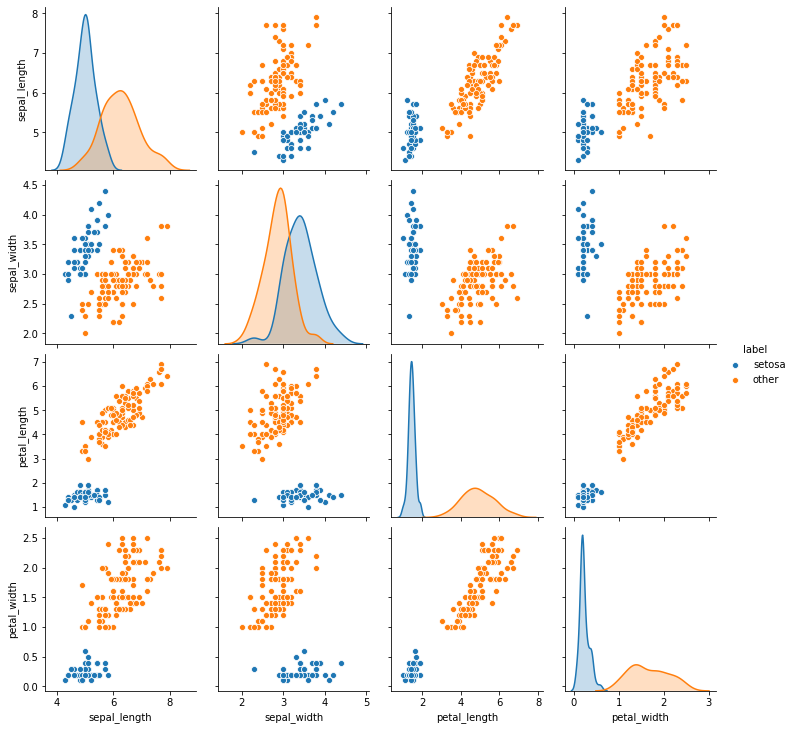
\includegraphics[scale=0.35]{iris_pairs} \\
%    \caption{This is an example figure}
%    \label{fig:my_label}
%\end{figure}
\documentclass[]{hdsr}
\usepackage{amsmath,amsthm,amssymb,mathrsfs,upgreek,stmaryrd,dsfont,tikz-cd,mathtools}
\usepackage[utf8]{inputenc}
\usepackage{babel}



\newtheorem{theorem}{Teorema}[section]
\newtheorem{corollary}{Corolario}[theorem]
\newtheorem{lemma}[theorem]{Lema}
\theoremstyle{definition}
\newtheorem{definition}{Definición}[section]

\newcommand{\R}{\mathbf{}{R}}
\newcommand{\P}{\mathbf{P}}
\newcommand{\N}{\mathbf{N}}
\begin{document}
\begin{center}
  \title{Movimiento Browniano}
  \maketitle
\end{center}

\vspace*{0.15in}

\section{Movimiento Browniano como una función aleatoria}

    \subsection{Procesos estocásticos}
    \begin{definition}
        Un \textit{Proceso estocástico} es una colección de variables aleatorias \( \{X_t(s): t \in T, s \in S \} \), donde $T$ es un conjunto de índices y $S$ es el espacio en común de las variables aleatorias. Por lo general se denota a $t$ como el tiempo así $X_t$ representa el estado del proceso en un tiempo $t \in T$.
    \end{definition}
    \begin{definition}
        Denotamos, para cada $s \in S$ fijo, a  $X_t(s)$ como la \textit{función de muestreo} o \textit{realización del proceso estocástico}.
    \end{definition}
    De acuerdo al espacio de muestreo $S$ denotamos:
    \begin{definition} Denotamos a un proceso estocástico como 
        \begin{itemize}
            \item \textit{Proceso estocástico discreto} si  $S=1,2,3...$.
            \item \textit{Proceso estocástico real-valuado} si \( S= (-\infty,\infty) \).
            \item \textit{Proceso estocástico $k$-vectorial} si $S$ es un espacio euclidiano de dimensión $k$.
        \end{itemize}
    \end{definition}
    
    \subsection{Construcción de Paul Lévy}
    \begin{definition}
        Un proceso estocástico real-valuado \( \{ B(t): t\geq 0 \} \) se dice un \textit{Movimiento Browniano lineal} con comienzo en $x \in \R$ si:
        \begin{itemize}
            \item \(B(0)=x\) (si $x=0$, se denomina \textit{movimiento browniano estándar},
            \item Tiene incrementos positivos,
            \item Para todo $t \geq 0$ y $h>0$, \( B(t+h)-B(t) \) tiene distribución normal con varianza $h$ y valor esperado $0$.
            \item \( t \mapsto B(t) \) es casi siempre continua.
        \end{itemize}
    \end{definition}
    \begin{theorem}
        El movimiento Browniano estándar existe.
    \end{theorem}
    \begin{proof}
        Sea \( (\Omega, \mathcal{A}, \P ) \) un espacio de probabilidad. Sea \( \{Z_t:t \in D \} \) una colección de variables aleatorias independientes con distribución normal estándar donde \(D=\cup_{n=0}^{\infty}D_n \) definidos por 
        \[
            D_n = \left\{ \frac{k}{2^n}: 0\leq k \leq 2^n \wedge k \in \N \right\}
        \].
        Por inducción, considere la variable aleatoria dada por  
        \[
            B(0)=0, B(1)=Z_1, B(d)=\frac{B(d-\frac{1}{2^n}+B(d+\frac{1}{2^n})}{2}+\frac{Z_d}{2^(n+1)/2}
        \]
        Note que:
        \begin{enumerate}[(1)]
            \item Para todo \( s<t \in D_0={0,1} \), \(B(t)-B(s)=B(1)-B(0)=B(1)=Z_1 \) tiene distribución normal donde su valor esperado es 0 y su varianza es \(t-s=1-0=1\).
            \item \((B(d):d\in \D_n )= (B(d):d \in D_0)= (B(0),B(1))\) y \((Z_t: t \in D\setminus D_n )=(Z_t:t\in D\setminus{0,1}\) son independientes.
        \end{enumerate}
        Suponga que estas propiedades se cumplen para todo \( n-1 \in \n \), queremos ver que se cumplan para $n$.
        \begin{enumerate}[(1)]
            \item Para todo \( r<s<t \in D_n \), \(B(t)-B(s)\) tiene distribución normal con valor esperado 0 y varianza \(t-s\).w
        \end{enumerate}
    \end{proof}
    
    
    \subsection{Propiedades de invarianza del moviemiento Browniano}
    
    \begin{lemma}[Scaling invariance]
        Suponga que \( \{ B(t):t\geq0\} \) es un movimiento browniano estándar y sea $a>0$. Entonces, el proceso \( \{X(t):t\geq0\} \) dado por \(X(t)= \frac{1}{a}B(a^2t) \) también es un movimiento browniano estándar. 
    \end{lemma}
    \begin{lemma}[Time inversion]
        Suponga que \(\{ B(t):t\geq0 \}\) es un movimiento browniano estándar. Entonces el proceso \( \{X(t): t\geq 0\}\) definido por 
        \[
            X(t) = \left\{
                            \begin{array}{lr}
                                0 & t=0 \\
                                tB\left(\frac{1}{t}\right) & t>0
                            \end{array}\right.
        \]
        Es un movimiento Browniano estándar.  
    \end{lemma}
    
    \begin{corollary}[Ley de los grandes números]
        Casi siempre 
        \[
            lim_{t\to \infty}\frac{B(t)}{t}=0
        \]
    \end{corollary}
\end{document}
